\section{Configuration Similarity}
\label{sec:similarity}

Previous measurement students have found extensive use of templates in
configurations from actual networks. Thus, we expect a network's
configurations to share a common set of tokens and statements. To confirm this
hypothesis, we split the configurations of a large university network
(University A in Table~\ref{tab:datasets}) into tokens---each keyword and
identifiers (e.g., interface names, VLAN numbers, IP prefixes, etc.) is
considered a token. For each device, we measured the fraction of
tokens and statements (i.e., lines of configuration) that existed in at least
one other device's configuration.

\begin{figure}
	\centering
	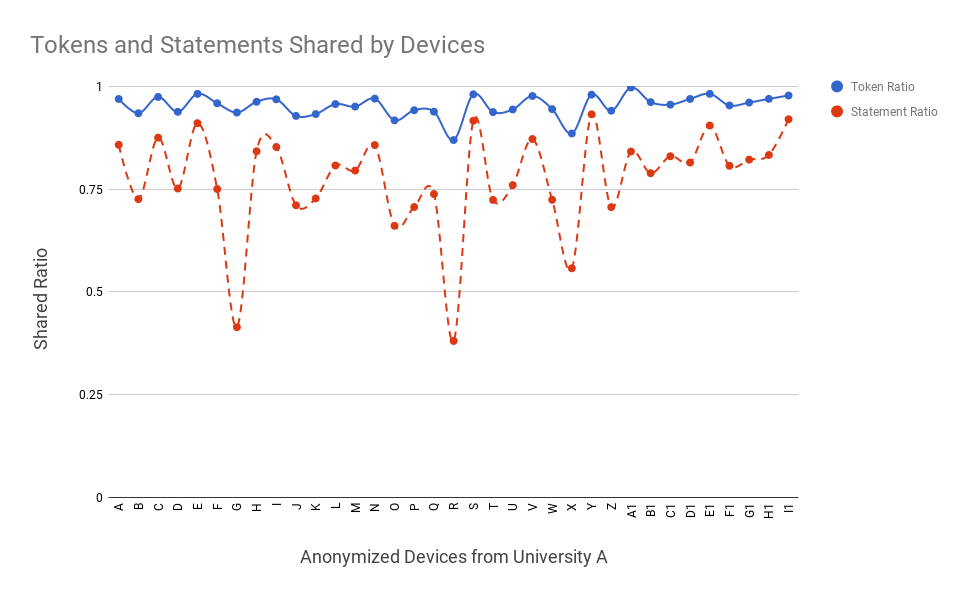
\includegraphics[width=\columnwidth]{chart.png}
	\caption{Token and statement similarity for Univ-A}
    \vspace{-2em}
    \label{fig:chart}
\end{figure}

As shown in Figure~\ref{fig:chart}, almost all configurations were composed of
the same set of unique tokens. The tokens that are not shared between
configurations are primarily IP prefixes. Moreover a large fraction of
statements appeared in another device's configuration. These observations
indicate that most of a device's configuration could be constructed from
existing configurations.
